\startcontents[localtoc]
\printcontents[localtoc]{}{0}{\subsection*{Contents}\setcounter{tocdepth}{2}}



\phantomsection
\addcontentsline{toc}{section}{Generate sampled data}
\subsubsection*{Generate sampled data}



Three quantities have to be prepared: time series \texttt{t} and signal \texttt{y},
representing 2000 samples of sinus waveform of nominal frequency 49.77 Hz, nominal
amplitude 1 V and nominal phase 0 rad, sampled with sampling period 0.25 ms.
Signal simulates non-coherent sampling.

\begin{lstlisting}
f = 49.77;
A = 1;
N = 2000;
fs = 4000;
Ts = 1/fs;
Sampled.t.v = [0 : N-1] * Ts;
Sampled.y.v = A*sin(2 * pi * f * Sampled.t.v);
\end{lstlisting}


\phantomsection
\addcontentsline{toc}{section}{Signal frequency estimate}
\subsubsection*{Signal frequency estimate}



Get estimate of signal frequency to be coherent after resampling. For
example, algorithm PSFE can be used:

\begin{lstlisting}
Estimate = qwtb('PSFE', Sampled);
Sampled.fest.v = Estimate.f.v;
\end{lstlisting}
\begin{lstlisting}[language={},xleftmargin=5pt,frame=none]
QWTB: no uncertainty calculation
QWTB: PSFE wrapper: sampling time was calculated from time series

\end{lstlisting}


\phantomsection
\addcontentsline{toc}{section}{Call algorithm}
\subsubsection*{Call algorithm}

\begin{lstlisting}
Resampled = qwtb('SplineResample', Sampled);
\end{lstlisting}
\begin{lstlisting}[language={},xleftmargin=5pt,frame=none]
QWTB: no uncertainty calculation
QWTB: SplineResample wrapper: sampling time was calculated from time series

\end{lstlisting}


\phantomsection
\addcontentsline{toc}{section}{Get spectra}
\subsubsection*{Get spectra}

\begin{lstlisting}
SpectrumNonCoherent = qwtb('SP-WFFT', Sampled);
SpectrumResampled = qwtb('SP-WFFT', Resampled);
\end{lstlisting}
\begin{lstlisting}[language={},xleftmargin=5pt,frame=none]
QWTB: no uncertainty calculation
QWTB: SP-WFFT wrapper: sampling frequency was calculated from time series
warning: QWTB: value of quantity `y` is column vector, it was automatically transposed.
warning: called from
    qwtb>check_gen_datain at line 969 column 25
    qwtb>check_and_run_alg at line 342 column 16
    qwtb at line 114 column 47
    publish>eval_code_helper at line 1079 column 8
    publish>eval_code at line 995 column 30
    publish at line 402 column 9
    all_algs_examples2tex at line 51 column 5
 
QWTB: no uncertainty calculation

\end{lstlisting}


\phantomsection
\addcontentsline{toc}{section}{Compare estimated amplitudes}
\subsubsection*{Compare estimated amplitudes}

\begin{lstlisting}
printf('Frequency and amplitude of main signal component.\n');
printf('Simulated:                      f = %.2f, A = %.5f\n', f, A)
id = find(SpectrumNonCoherent.A.v == max(SpectrumNonCoherent.A.v));
printf('As estimated\n')
printf('Non coherent sampling and FFT:  f = %.2f, A = %.5f\n', SpectrumNonCoherent.f.v(id), SpectrumNonCoherent.A.v(id));
id = find(SpectrumResampled.A.v == max(SpectrumResampled.A.v));
printf('Resampled to coherent and FFT: f = %.2f, A = %.5f\n', SpectrumResampled.f.v(id), SpectrumResampled.A.v(id));
\end{lstlisting}
\begin{lstlisting}[language={},xleftmargin=5pt,frame=none]
Frequency and amplitude of main signal component.
Simulated:                      f = 49.77, A = 1.00000
As estimated
Non coherent sampling and FFT:  f = 50.00, A = 0.97996
Resampled to coherent and FFT: f = 49.77, A = 1.00000

\end{lstlisting}


\phantomsection
\addcontentsline{toc}{section}{Plot}
\subsubsection*{Plot}

\begin{lstlisting}
hold on
semilogy(f, A, 'xk')
semilogy(SpectrumNonCoherent.f.v, abs(SpectrumNonCoherent.A.v), '-k')
semilogy(SpectrumResampled.f.v, abs(SpectrumResampled.A.v), '-r')
hold off
xlabel('Frequency (Hz)')
ylabel('Signal amplitude')
legend('Simulated signal', 'FFT spectrum', 'Resampled and FFT spectrum')
title('Signal spectra')
\end{lstlisting}
\begin{center}
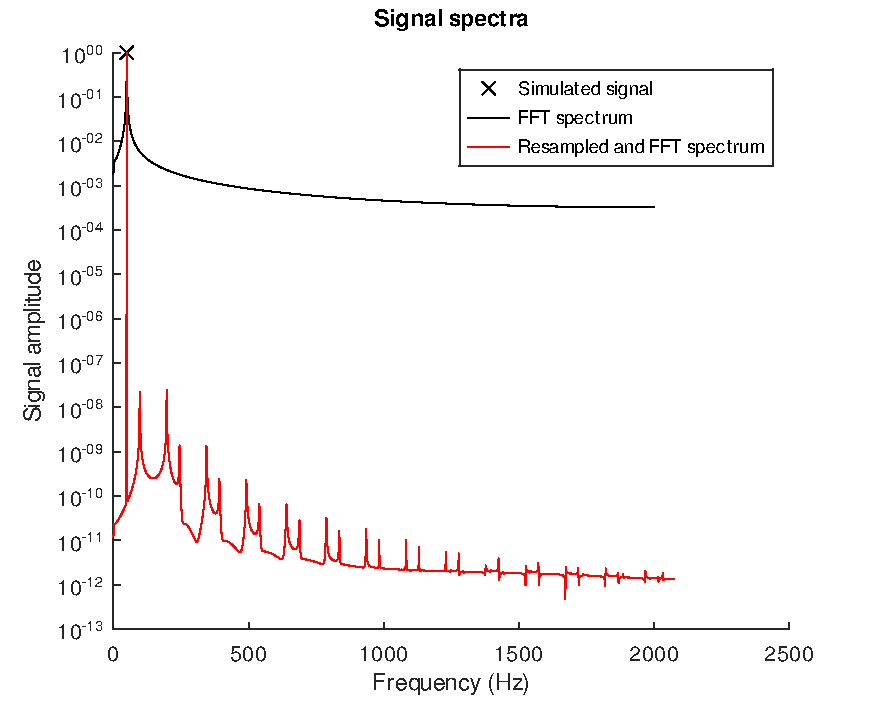
\includegraphics[width=0.7\textwidth]{algs_examples_published/SplineResample_alg_example-1.pdf}
\end{center}


\stopcontents[localtoc]
